\subsection{Methode Charakteristiken}

\textbf{Wichtig:} Als Anfangsbedingungen dürfen \textbf{keine} Charakteristiken verwendet werden, sonst ist die Charakteristik die Lösung (anstatt Fläche ergibt sich eine Kurve).\\
\textbf{Wichtig:} Die Charakteristik darf den Rand nur einmal durchlaufen.\\
Nützlich für Quasilineare PDGL 1.Ordnung. Wenn Separation möglich ist, sollte diese (einfachere) Methode verwendet werden.\\

Ausgangslage:
\[
    a(x,y,u)\cdot\partFrac{u}{x}+b(x,y,u)\cdot\partFrac{u}{y}-c(x,y,u)=0
\]
Charakteristik:
\[
    \frac{d}{dt} \begin{bmatrix} x(t) \\ y(t) \\ u(t) \end{bmatrix}
    = \begin{bmatrix} a(x,y,u) \\ b(x,y,u) \\ c(x,y,u) \end{bmatrix}
\]


\begin{tabular}{ll}
Gebiet:& $\Omega\{\ldots|x>0, \text{alle }y\}$\qquad Randbedingung: $u(0,y_0)=g(y_0)$\\
Vektorielle Schreibweise:& $\begin{bmatrix}
    a(x,y,u)\\ b(x,y,u)\\ c(x,y,u)
    \end{bmatrix}
\underset{\overrightarrow{n}\text{: Normale auf Fläche}}{\underbrace{\begin{bmatrix}
\partFrac{u}{x} & \partFrac{u}{y} & -1
\end{bmatrix}}}=0 $ \\[1cm]
Tangenten:& $\overrightarrow{t}_x=\begin{bmatrix}1\\0\\ \partFrac{u}{x}\end{bmatrix}\qquad 
			\overrightarrow{t}_y=\begin{bmatrix}0\\1\\ \partFrac{u}{y}\end{bmatrix}\qquad \overrightarrow{n} \bullet \overrightarrow{t_x} = 0 \qquad \overrightarrow{n} \bullet \overrightarrow{t_y} = 0 \qquad \overrightarrow{t_x} \bullet \overrightarrow{t_y} = \overrightarrow{n}$\\[1cm]

Lösungsweg: & Für jeden Anfangspunkt $\begin{bmatrix} 0\\y_0\\g(y_0)\end{bmatrix}$ finde eine Charakteristik, diese nach $x$, $y$ auflösen.
\end{tabular}

\paragraph{Randbedingungen}
Eine Lösungsfunktion $u(x,y)$ muss von Charakteristiken überdeckt werden.
Die Lösung wird nun durch die Randwerte bestimmt.

\begin{minipage}{10cm}
    Für das dargestellte Gebiet $\Omega$ sind verschiedene Fälle möglich:
    \begin{enumerate}
        \item Randwerte am \emph{linken} und \emph{rechten} Rand sind vorgegeben.
        Ein Gebiet in der Mitte ist nicht bestimmt.
        \item Randwerte am \emph{oberen} und \emph{unteren} Rand sind vorgegeben.
        Ein Teil des Gebiets ist überbestimmt.
        \item Randwerte am \emph{linken} und \emph{unteren} Rand sind vorgegeben.
        Funktion ist eindeutig bestimmt (aber nicht unbedingt überall differenzierbar).
    \end{enumerate}
    Die Lösung ist also nicht für alle Randwerte bestimmbar. \newline
    Wenn sich zwei Charakteristiken treffen $\rightarrow$ Singularität
\end{minipage}
\hspace{0.5cm}
\begin{minipage}{8cm}
    \centering
    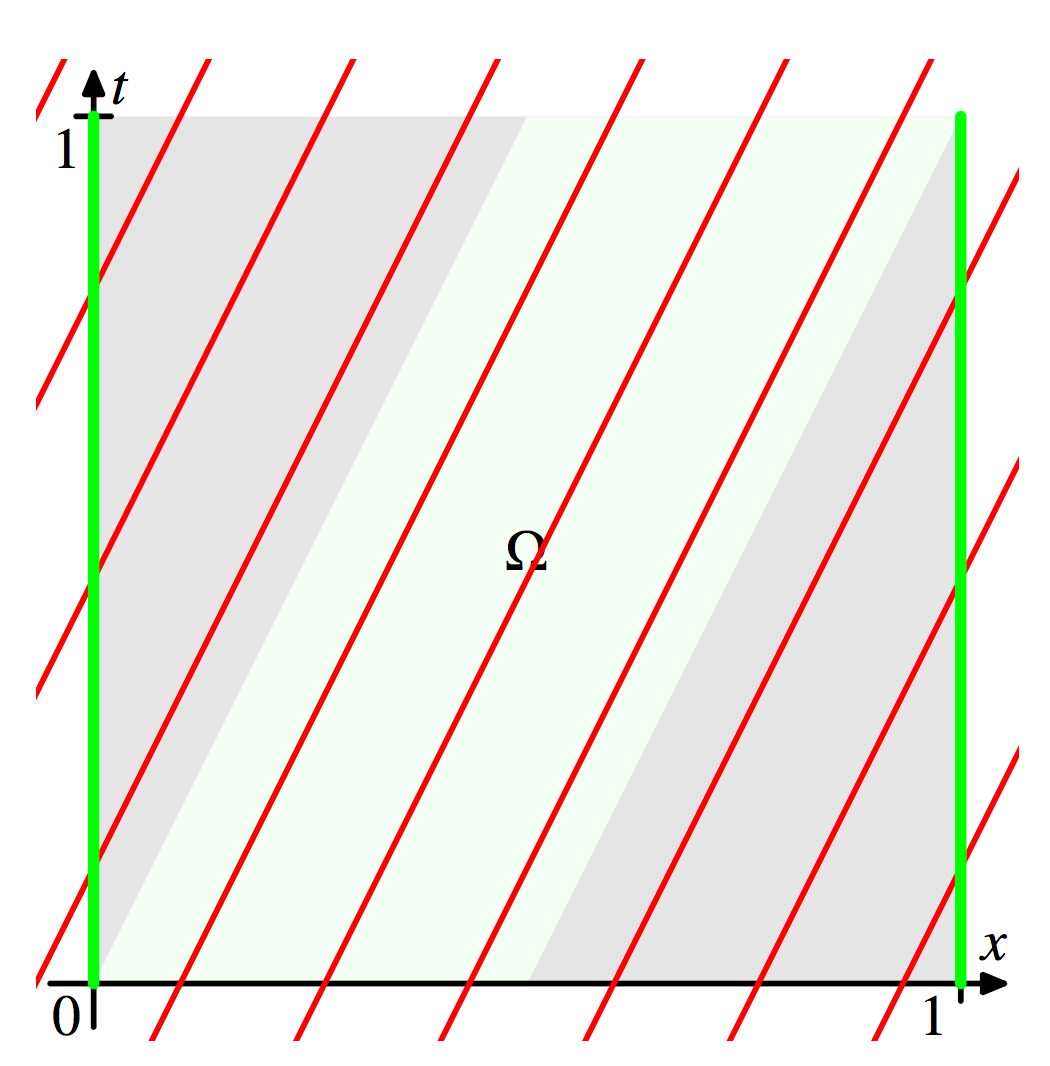
\includegraphics[width=6cm]{Content/01_theory/charakteristiken_randwerte.png}
\end{minipage}

\paragraph{Beispiel:}~\\
\begin{enumerate}
	\item PDGL mit Randbedingungen und Definitionsbereich: $\partFrac ux+2\partFrac uy=3$, \; $u(0,y)=g(y)=\sin(y) \Rightarrow u(0,y_0) = g(y_0) = \sin(y_0)$\\
	Terme in Matrixschreibweise: $\begin{bmatrix}a\\b\\c\end{bmatrix}=\begin{bmatrix}1\\2\\3\end{bmatrix}$
	\item Charakteristiken ausrechnen PDGL $\rightarrow$ DGL: 	$\frac {d}{dt}\begin{bmatrix}x(t)\\y(t)\\u(t)\end{bmatrix}=\begin{bmatrix}1\\2\\3\end{bmatrix}$
	\item DGL's lösen (für Standard-DGL's, siehe \ref{sec:dgls} auf Seite \pageref{sec:dgls}.): 
	$\begin{bmatrix}x\\y\\u\end{bmatrix}=\begin{bmatrix}1t+x_0\\2t+y_0\\3t+u_0\end{bmatrix}$
	\item Anfangsbedingungen einsetzen: $\begin{bmatrix}x\\y\\u\end{bmatrix}=\begin{bmatrix}1t+x_0\\2t+y_0\\3t+u_0\end{bmatrix}\Bigg|_{t=0}=
	\begin{bmatrix}x_0\\y_0\\u_0\end{bmatrix}=\begin{bmatrix}0\\y_0\\\sin(y_0)\end{bmatrix}$\\
	Lösung der DGL ist: $\begin{bmatrix}x\\y\\u\end{bmatrix}=\begin{bmatrix}1\\2\\3\end{bmatrix}\cdot t+ \begin{bmatrix}0\\y_0\\\sin(y_0)\end{bmatrix}$\\
	
	\item Eliminieren aller Variablen ausser $u,x,y$: $u=3x+\sin(y-2x)$
	\item Kontrolle:
	Resultat ($u=3x+\sin(y-2x)$) ableiten und in Aufgabenstellung einsetzen $\partFrac ux+2\partFrac uy=3$ und schauen ob es erfüllt.
	
\end{enumerate}
